\chapter{Resultados}
\label{cap:resultados}
\phantom{0}

%Este capítulo apresenta e discute os resultados experimentais de cada etapa do método proposto. O procedimento de avaliação dos resultados foi o seguinte: 1) preparação da base de imagens e configuração experimental; 2) resultados iniciais da segmentação de rins e tumores renais; 3) reconstrução dos tumores renais; e 4) resultados finais da segmentação de rins e tumores renais.

Este capítulo apresenta os resultados experimentais de cada etapa do método proposto. Primeiramente, é apresentada a base de imagens que foi usada. Em seguida, é mostrada a avaliação dos resultados, com os seguintes procedimentos: 1) configuração experimental; 2) resultados gerais do método proposto; 3) resultados iniciais da segmentação de rins; 4) resultados iniciais de candidatos a tumores renais; 5) reconstrução dos tumores renais; e 6) resultados finais da segmentação de rins. 

\section{Base de Imagens}
\label{sec:conjunto-dados}

Neste trabalho, a base de imagens usada para realizar os experimentos foi de um desafio denominado KiTS19. Este desafio teve como objetivo acelerar a pesquisa e desenvolver novos recursos nefrométricos para auxiliar no prognóstico do tumor renal e no planejamento do tratamento; e também a criação de métodos confiáveis de segmentação semântica para rim e tumor renal~\cite{1904.00445}.

A base de imagens KiTS19 consiste em TCs de pacientes que foram submetidos a nefrectomia parcial ou radical para um ou mais tumores renais. Os exames foram coletados pelo Centro Médico da Universidade de Minnesota (\textit{University of Minnesota Medical Center}) entre 2010 e 2018. De acordo com o desafio, a base de imagens contém 300 TCs, divididos em 210 TCs para treinamento e validação e os 90 restantes para avaliar o desempenho do modelo. Para o conjunto de treinamento e validação, o desafio disponibilizou máscaras de segmentação semântica (anotações) e foram esses conjuntos de imagens que foram usados para realizar os experimentos desta tese. Essas anotações foram fornecidas por estudantes de medicina que realizaram segmentações manuais sob a supervisão dos radiologistas e patologistas cirúrgicos (Drs. Christopher Weight e Niranjan Sathianathen). Isso ajudou na localização precisa dos tumores para evitar classificação incorreta como cistos que também podem estar presentes~\cite{1904.00445}.

Todos os pacientes foram tratados por urologistas em um único centro de atendimento e mais da metade dos exames foram adquiridos em mais de 50 instituições de referência. Para cada instituição, uma variedade de protocolos de aquisição é aplicada. Isso torna a base de imagens KiTS19 diversa em termos de dimensões de \textit{voxel}, tempo de contraste, assinatura de tabela e campo de visão do scanner. Além disso, ajuda a minimizar algumas preocupações sobre a validade externa de um coorte retrospectivo\footnote{O pesquisador colhe informação pregressa dos fatores de exposição e acompanha por um período de tempo os indivíduos~\cite{CAMARGO2019}.} de uma única instituição, como o KiTS19~\cite{HELLER2021101821}.

Cada volume de TC (imagens e máscaras) foi fornecido no formato NIFTI~\cite{NIFTI}. Todos os volumes têm resolução $512\times512$ em escala de cinza, e o número de fatias varia de 29 a 1059. O método proposto tem como objetivo segmentar os rins e também os tumores renais entre os cistos presentes, o que é um desafio devido às semelhanças. A Figura~\ref{fig:ExImagemEMascara} ilustra um exemplo de fatia de um volume, que contém as marcações: rins (azul) e tumores (vermelho).

\begin{figure}[ht!]
    \centering
    \caption{Informações da base de imagens: fatia com marcações de rins (azul) e tumores (vermelho).}
    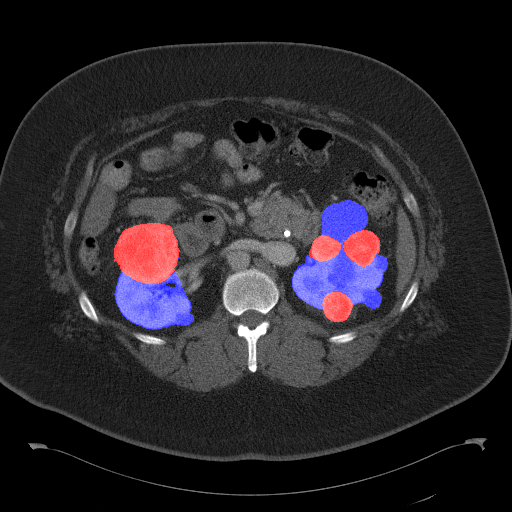
\includegraphics[width=0.55\textwidth]{figuras/exemplo-dataset.png}
    \legend{Fonte: Elaborado pela autora.}
    \label{fig:ExImagemEMascara}
\end{figure}

\subsection{Distribuição Proporcional da Base de Imagens}
\label{sec:res-distribuicao-proporcional-dataset}

Esta seção apresenta o resultado da aplicação do método para distribuição proporcional da base de imagens. Para realizar os experimentos, foi usada a base de imagens KiTS19, na qual o conjunto de teste (31 TCs) foi inicialmente selecionado aleatoriamente entre os 210 TCs disponíveis. Os demais exames de TC foram usados como entrada para o método, seguindo as três etapas principais (Seção~\ref{sec:distribuicao-proporcional-dataset}): (1) reamostrar os exames; (2) extrair \textit{deep features}; e (3) agrupar.

É importante mencionar que antes de reamostrar os exames, a quantidade de fatias de tumores renais em cada exame variou de 3 a 256. A primeira etapa, foi realizada a técnica de reamostragem dos exames de TC. Na qual, obteve-se o valor médio de fatias de exames de TC por meio da operação média, que consistiu em calcular a quantidade total de fatias de tumores (4.927) contidos no conjunto de treino e validação, e dividir pela quantidade de exames totais (179). Como resultado, o valor médio foi de 27 fatias. Por fim, foi aplicada a técnica de reamostragem e todos os exames passaram a ter 27 fatias.

Na segunda etapa, são extraídas as \textit{deep features} dos exames reamostrados. A Tabela~\ref{tab:numero-caracteristicas} mostra o número de características extraídas dos exames para cada modelo descrito na Seção~\ref{sec:distribuicao-proporcional-dataset}.

\begin{table}[!ht]
\caption{Total de características extraídas em cada modelo de CNN.}
\label{tab:numero-caracteristicas}
\centering
\begin{tabular}{c|c|c}
\hline
Modelo     & N° de características por fatia & Total (27 fatias) \\ \hline
ResNet-18  & 512                             & 13.824             \\ \hline
ResNet-34  & 512                             & 13.824             \\ \hline
ResNet-101 & 2.048                            & 55.296             \\ \hline
VGG-11     & 1.000                            & 27.000             \\ \hline
VGG-16     & 1.000                            & 27.000             \\ \hline
DPN-131    & 2.688                            & 72.576             \\ \hline
Xception   & 2.048                            & 55.296             \\ \hline
\end{tabular}
\end{table}

Na terceira etapa, as características extraídas por cada modelo são usadas para realizar o agrupamento de dados. A Tabela~\ref{tab:melhores-grupos} apresenta os modelos, o melhor grupo encontrado dentre os K-grupos (2 a 20) e o valor da inércia. Dentre eles, o modelo ResNet-34, que tem o valor seis representando o melhor grupo, foi o escolhido por apresentar a menor inércia (49.158).

\begin{table}[!ht]
\caption{Melhores grupos e suas inércias encontrados para os modelos usando o método do cotovelo.}
\label{tab:melhores-grupos}
\centering
\begin{tabular}{c|c|c}
\hline
Modelo     & N° ótimo de grupos & Inércia       \\ \hline
ResNet-18  & 6                  & 55.260        \\ \hline
\rowcolor[HTML]{C0C0C0} 
ResNet-34  & 6                  & 49.158        \\ \hline
ResNet-101 & 5                  & 83.542        \\ \hline
VGG-11     & 6                  & 248.324.688   \\ \hline
VGG-16     & 8                  & 134.276.912   \\ \hline
DPN-131    & 7                  & 5.828.450.304 \\ \hline
Xception   & 6                  & 2.972.436     \\ \hline
\end{tabular}
\end{table}

A Figura~\ref{fig:distribuicao-proporcional} apresenta o gráfico com o número de exames para cada um dos grupos encontrados. Finalmente, os casos (exames) de cada um dos seis grupos gerados pelo método proposto foram selecionados aleatoriamente e distribuídos proporcionalmente entre os conjuntos de dados de treinamento (148 exames) e validação (31 exames).

\begin{figure}[!ht]
    \centering
    \caption{Grupos de tumores encontrados com a aplicação do método a partir dos conjuntos de treinamento e validação.}
    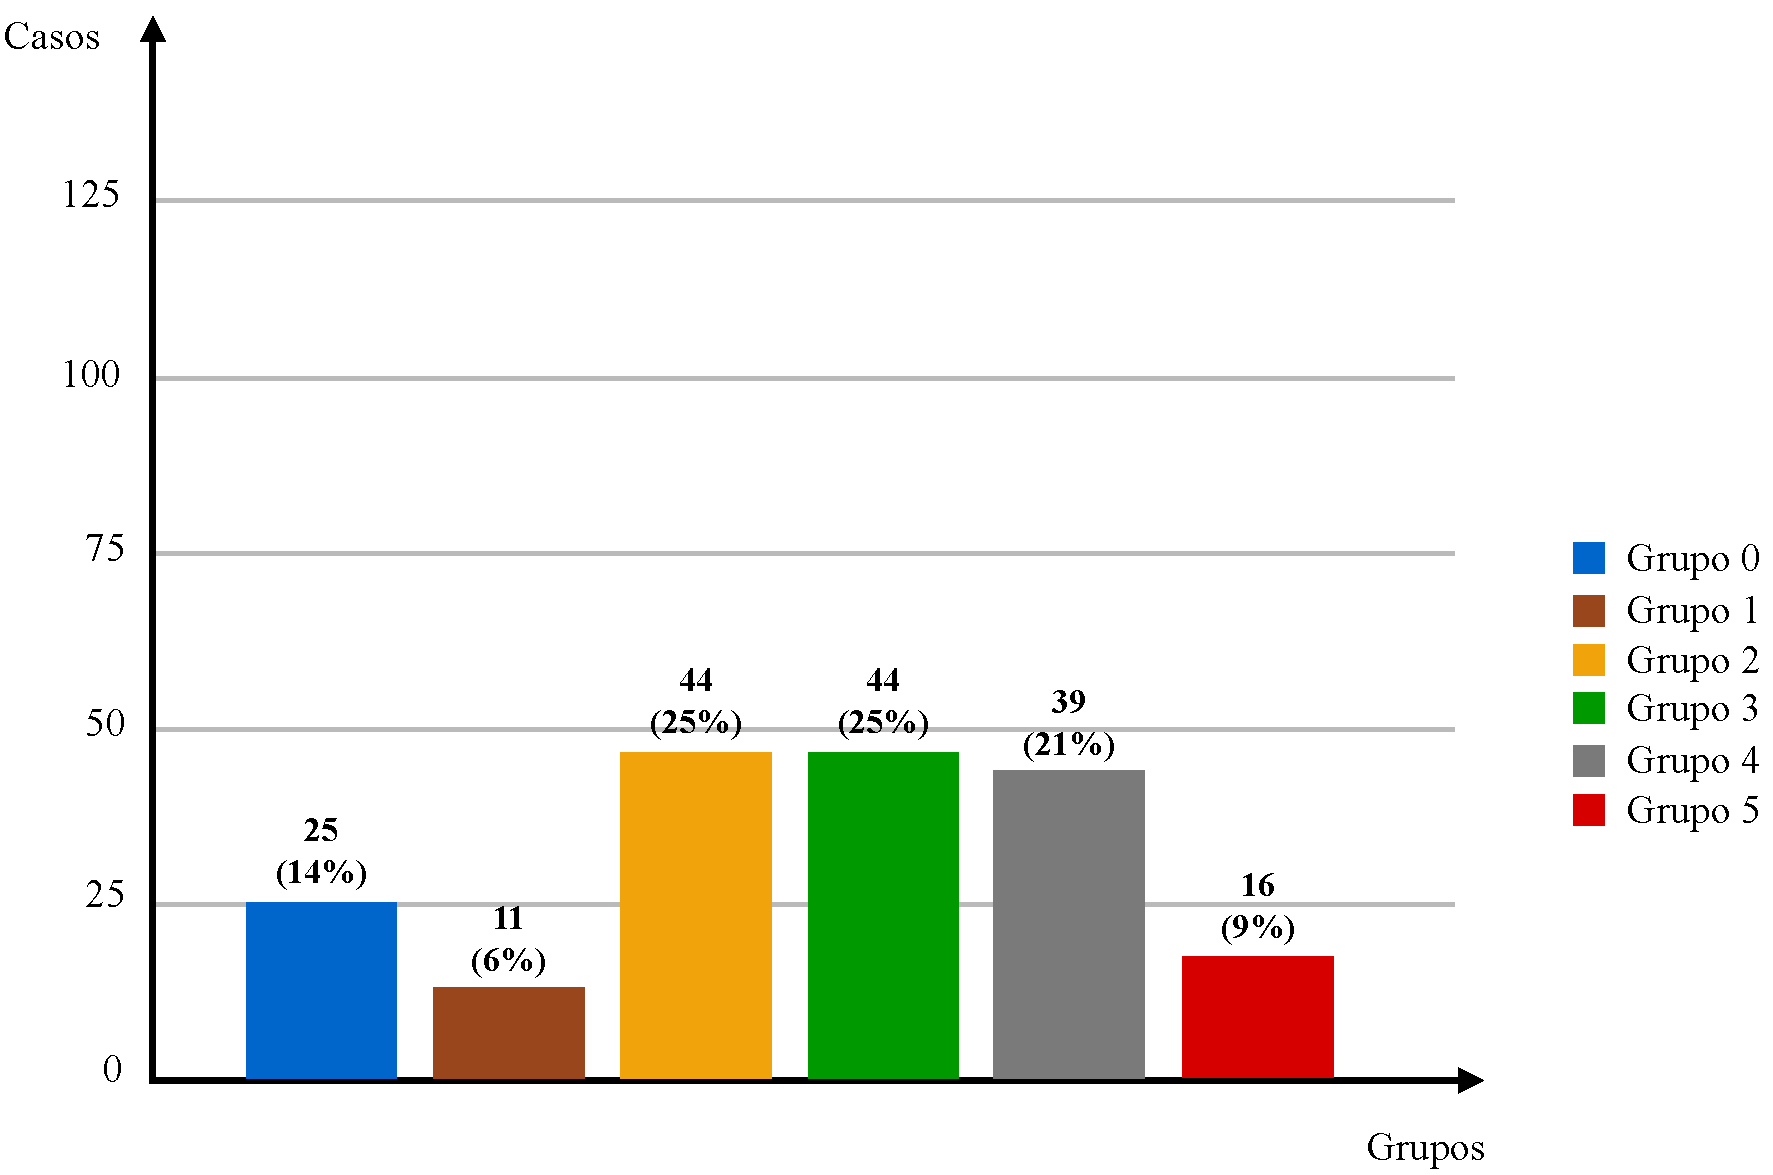
\includegraphics[width=0.75\textwidth]{figuras/distribuicao-proporcional.pdf}
    \legend{Fonte: Elaborado pela autora.}
    \label{fig:distribuicao-proporcional}
\end{figure}

\subsection{Preparação da Base de Imagens}
\label{sec:preparacao-conjunto-dados}

Inicialmente, os volumes de TC foram pré-processados (Seção~\ref{sec:pré-processamento}) antes de serem usados como entrada para a ResUNet 2.5D (Seções~\ref{sec:metodo-segmentacao-dos-rins-ResUNet} e \ref{sec:metodo-candidatos-tumores-renais-regiao-abdominal}) e DeepLabv3+ 2.5D (Seção~\ref{sec:metodo-candidatos-tumores-renais-regiao-renal}). Para fins de teste e validação, foram separados aproximadamente 148 (70\%) volumes de TC para treinamento, 31 (15\%) para validação e 31 (15\%) para teste do conjunto de 210 TCs disponíveis. Inicialmente, o conjunto de teste foi selecionado aleatoriamente (31 casos), e com os casos restantes (179 casos), uma distribuição proporcional foi feita para separar os casos entre os conjuntos de treinamento e validação, conforme descrito na Seção~\ref{sec:res-distribuicao-proporcional-dataset}. Além disso, foi realizado um balanceamento de fatias para cada modelo de aprendizado profundo (Seções~\ref{sec:treinamento-ResUNet}, \ref{sec:treinamento-DeepLabv3+} e \ref{sec:metodo-candidatos-tumores-renais-regiao-abdominal}).

\section{Configuração Experimental}
\label{sec:configuracao-experimental}

O método proposto foi implementado usando a linguagem de programação Python e principalmente a biblioteca de aprendizado profundo Pytorch~\cite{NEURIPS2019_9015}. O computador usado nos experimentos consistia em uma CPU Intel Core i7-7700K 4.20GH, 16 GB de RAM e placa de vídeo Nvidia GeForce GTX 1080-Ti, executado no sistema operacional Windows 10.

O critério de parada nos modelos de treinamento foi usando a técnica early stop~\cite{brownlee2018better}, que consiste em parar o treinamento da rede quando a métrica monitorada (o valor da função de perda nos dados de validação) parasse de melhorar em 15 épocas. Os hiperparâmetros usados nos modelos tinham um tamanho de \textit{batch} igual a 8, função de perda Dice~\cite{dice1945}, otimizador estocástico Adam~\cite{adam2014} com uma taxa de aprendizagem inicial de 0,0001 com decaimento de 10\% se o valor da função de perda nos dados de validação não cair em 7 épocas, beta-1 0,9 e beta-2 0,999 (taxas de decaimento iniciais usadas ao estimar o primeiro e o segundo momentos do gradiente). Após a aplicar o algoritmo de otimização \textit{Tree of Parzen Estimators} (TPE) usando a biblioteca Hyperopt~\cite{bergstra2013making}, este foi o conjunto de hiperparâmetros que produziu os melhores resultados. O tempo de execução total de otimização foi de aproximadamente 4 semanas.

As métricas (Seção~\ref{sec:metricas-de-desempenho}) usadas para avaliar o desempenho do método proposto foram: coeficiente de similaridade Dice (Dice), índice de Jaccard (Jacc), acurácia (Acc), sensibilidade (Sen) e especificidade (Esp). Além disso, foram realizados testes de significância\footnote{Teste de significância é um procedimento estatístico que permite tomar uma decisão entre duas ou mais hipóteses (rejeitar ou não rejeitar), usando os dados observados de um determinado experimento~\cite{statistical1982, zou2003}.} das etapas do método.

\section{Resultados Gerais do Método Proposto}
\label{sec:resultados-metodo-proposto}

Nesta seção, são apresentados os resultados obtidos em cada etapa do método proposto. Para que o método fosse validado, os conjuntos de treino, validação e teste foram distribuídos 5 vezes usando os mesmos procedimentos descritos na Seção~\ref{sec:preparacao-conjunto-dados}. Posteriormente, em cada etapa do método, a CNN foi executada 5 vezes (5-\textit{folds}) usando os conjuntos de dados mencionados. Essa prática tem a finalidade de verificar a eficiência do método independentemente do conjunto de dados avaliado, garantindo que o método não seja tendencioso~\cite{burman1989comparative}. % Também evitar o problema de overfitting, uma vez que todo o conjunto de dados foi treinado pelo menos uma vez nos folds~\cite{burman1989comparative}.

A Tabela~\ref{tab:resultados-iniciais-metodo} apresenta os resultados dos 5-\textit{folds} para cada uma das etapas do método proposto, seguido da média e desvio padrão. Por fim, é mostrado o tempo de treinamento para cada época das abordagens. Analisando os resultados individuais, pode-se perceber que a segmentação dos rins apresentou bons resultados iniciais, atingindo uma média de Dice igual a 96,37\% com desvio padrão de 1,20. Nos candidatos a tumores renais, obtiveram-se resultados médios de 78,49\% de Dice e desvio de 2,06, levando em consideração que os candidatos a tumores renais foram segmentados dentro da região renal obtidas pela segmentação inicial dos rins.

\begin{table}[!ht]
\caption{Resultados iniciais das etapas do método proposto.}
\label{tab:resultados-iniciais-metodo}
\centering
\resizebox{\columnwidth}{!}{
\begin{tabular}{c|c|c|c|c|c}
\hline
Segmentação Inicial                                                                                        & Dice(\%)     & Jacc(\%)     & Acc(\%)      & Sen(\%)      & Esp(\%)      \\ \hline
\multirow{6}{*}{Rins}                                                                                      & 96,77        & 93,80        & 99,93        & 97,58        & 99,96        \\ \cline{2-6} 
                                                                                                           & 96,54        & 93,46        & 99,90        & 96,08        & 99,97        \\ \cline{2-6} 
                                                                                                           & 94,40        & 91,10        & 99,90        & 93,31        & 99,97        \\ \cline{2-6} 
                                                                                                           & 97,65        & 95,43        & 99,96        & 97,55        & 99,98        \\ \cline{2-6} 
                                                                                                           & 96,52        & 93,74        & 99,94        & 95,82        & 99,98        \\ \cline{2-6} 
                                                                                                           & 96,37 ± 1,20 & 93,51 ± 1,55 & 99,93 ± 0,03 & 96,07 ± 1,74 & 99,97 ± 0,01 \\ \hline
\multirow{6}{*}{\begin{tabular}[c]{@{}c@{}}Candidatos a Tumores Renais\\ na Região Renal\end{tabular}}     & 81,02        & 69,66        & 99,93        & 80,52        & 99,97        \\ \cline{2-6} 
                                                                                                           & 80,10        & 68,65        & 99,90        & 81,66        & 99,97        \\ \cline{2-6} 
                                                                                                           & 77,72        & 67,36        & 99,89        & 82,02        & 99,96        \\ \cline{2-6} 
                                                                                                           & 77,68        & 67,55        & 99,95        & 78,10        & 99,97        \\ \cline{2-6} 
                                                                                                           & 75,91        & 63,91        & 99,95        & 74,98        & 99,98        \\ \cline{2-6} 
                                                                                                           & 78,49 ± 2,06 & 67,43 ± 2,17 & 99,93 ± 0,03 & 79,46 ± 2,94 & 99,97 ± 0,01 \\ \hline
\multirow{6}{*}{\begin{tabular}[c]{@{}c@{}}Candidatos a Tumores Renais\\ na Região Abdominal\end{tabular}} & 68,88        & 58,45        & 99,91        & 85,57        & 99,93        \\ \cline{2-6} 
                                                                                                           & 60,95        & 47,11        & 99,82        & 75,54        & 99,91        \\ \cline{2-6} 
                                                                                                           & 58,54        & 47,45        & 99,82        & 84,01        & 99,85        \\ \cline{2-6} 
                                                                                                           & 57,40        & 45,57        & 99,91        & 76,34        & 99,93        \\ \cline{2-6} 
                                                                                                           & 59,55        & 47,41        & 99,86        & 75,86        & 99,89        \\ \cline{2-6} 
                                                                                                           & 61,06 ± 4,56 & 49,20 ± 5,23 & 99,86 ± 0,05 & 79,46 ± 4,90 & 99,90 ± 0,04 \\ \hline
\multirow{6}{*}{\begin{tabular}[c]{@{}c@{}}Reconstrução de\\ Tumores Renais\end{tabular}}                  & 68,20        & 57,17        & 99,90        & 90,33        & 99,91        \\ \cline{2-6} 
                                                                                                           & 63,77        & 49,82        & 99,86        & 86,80        & 99,90        \\ \cline{2-6} 
                                                                                                           & 57,99        & 45,93        & 99,80        & 89,82        & 99,82        \\ \cline{2-6} 
                                                                                                           & 60,10        & 47,79        & 99,91        & 85,95        & 99,92        \\ \cline{2-6} 
                                                                                                           & 61,90        & 49,32        & 99,87        & 86,00        & 99,88        \\ \cline{2-6} 
                                                                                                           & 62,39 ± 3,89 & 50,01 ± 4,28 & 99,87 ± 0,04 & 87,78 ± 2,13 & 99,88 ± 0,04 \\ \hline
\end{tabular}
}
\end{table}

Na segmentação inicial de candidatos a tumores renais na região abdominal, foram obtidos resultados médios de 61,06\% de Dice com desvio padrão de 4,56. Porém, nesta etapa, a informação mais relevante é obtida pela métrica de sensibilidade, pois informa a quantidade percentual de tumores segmentados. Portanto, para a métrica sensibilidade, obtiveram-se resultados médios de 79,46\% com desvio padrão de 4,90. Por fim, a etapa de reconstrução de tumores renais apresentou resultados médios de 87,78\% de sensibilidade com desvio padrão de 2,13. Este resultado permite observar a importância desta etapa para a reconstrução de tumores renais, uma vez que porções consideráveis de tumores foram obtidas unindo os estágios a candidatos a tumores renais, adquirindo assim resultados de sensibilidade superiores aos estágios de candidatos a tumores renais.

Na Tabela~\ref{tab:resultados-finais-metodo} os resultados finais da segmentação de rins e tumores são mostrados. Pode-se observar que na segmentação final dos rins foram obtidos resultados superiores em todas as métricas em relação aos resultados iniciais dos rins. Na segmentação dos tumores também foram obtidos resultados superiores aos resultados iniciais dos candidatos a tumores renais. Para ambas as segmentações, a obtenção dos resultados superiores em relação aos resultados iniciais se deu devido a técnica de reconstrução robusta que acabou delimitando partes de regiões tumorais que também fazem partes de regiões renais. Além disso, as técnicas de pós-processamento potencializaram as segmentações por meio de seu refinamento.

\begin{table}[!ht]
\caption{Resultados finais do método proposto.}
\label{tab:resultados-finais-metodo}
\centering
\resizebox{\columnwidth}{!}{
\begin{tabular}{c|c|c|c|c|c}
\hline
Segmentação Final               & Dice(\%)     & Jacc(\%)     & Acc(\%)      & Sen(\%)      & Esp(\%)      \\ \hline
\multirow{6}{*}{Rins}           & 97,45        & 95,05        & 99,95        & 98,44        & 99,96        \\ \cline{2-6} 
                                & 97,47        & 95,11        & 99,93        & 97,27        & 99,98        \\ \cline{2-6} 
                                & 95,45        & 92,69        & 99,93        & 94,83        & 99,97        \\ \cline{2-6} 
                                & 97,80        & 95,70        & 100,00       & 97,90        & 99,98        \\ \cline{2-6} 
                                & 96,81        & 94,29        & 99,95        & 96,24        & 99,98        \\ \cline{2-6} 
                                & 97,00 ± 0,94 & 94,57 ± 1,16 & 99,95 ± 0,03 & 96,94 ± 1,43 & 99,97 ± 0,01 \\ \hline
\multirow{6}{*}{Tumores Renais} & 84,06        & 75,04        & 99,94        & 88,33        & 99,95        \\ \cline{2-6} 
                                & 81,70        & 70,47        & 99,92        & 86,80        & 99,96        \\ \cline{2-6} 
                                & 81,64        & 70,76        & 99,90        & 89,58        & 99,92        \\ \cline{2-6} 
                                & 81,95        & 71,29        & 99,95        & 85,71        & 99,97        \\ \cline{2-6} 
                                & 82,61        & 71,70        & 99,96        & 85,20        & 99,98        \\ \cline{2-6} 
                                & 82,39 ± 1,01 & 71,85 ± 1,84 & 99,94 ± 0,02 & 87,12 ± 1,82 & 99,96 ± 0,02 \\ \hline
\end{tabular}
}
\end{table}

Por fim, é importante mencionar que os resultados médios e seus desvios padrões comprovam que os resultados individuais fornecem fortes evidências que o método proposto é robusto, independentemente do conjunto de dados usado. Portanto, essa abordagem usando \textit{k-fold} permitiu fazer uma análise mais detalhada do método proposto em geral. No entanto, deve-se sempre ter muita cautela ao aplicar essa abordagem. Isso porque, dependendo do conjunto de dados, o custo computacional pode ser muito grande, pois o mesmo modelo é treinado em várias subdivisões.

Portanto, nas próximas seções, os resultados de cada etapa são apresentados com mais detalhes, além da realização de outros experimentos e análises usando outras abordagens. Para isso, foi selecionado o melhor \textit{fold} do método proposto considerando aquele que obteve o melhor resultado para os tumores, visto que a segmentação tumoral é mais delicada e propensa a ruídos. Portanto, o melhor \textit{fold} é o primeiro, e este foi usado como referência para descrever os resultados individuais, estudos de caso e comparação com trabalhos relacionados.

\section{Segmentação Inicial dos Rins}
\label{sec:segmentacao-inicial-rins}

Conforme descrito na Seção~\ref{sec:metodo-segmentacao-dos-rins-ResUNet}, o modelo ResUNet 2.5D foi usado para a segmentação inicial dos rins em imagens de TC. Para construir o modelo, foram usadas 23.670 fatias do conjunto de treino, 5.062 fatias do conjunto de validação e 5.506 fatias do conjunto de teste.

Para verificar a eficácia da abordagem 2.5D escolhida e a capacidade de uma melhor generalização, as abordagens 2D e 2.5D foram comparadas. Basicamente, o modelo ResUNet 2.5D foi substituído pelo modelo ResUNet 2D, usando as mesmas configurações descritas na Seção~\ref{sec:configuracao-experimental} e o balanceamento de fatias (Seção~\ref{sec:treinamento-ResUNet}). Em outras palavras, foram mostrados os resultados do método completo usando a abordagem 2D e a 2.5D em cada etapa do método. Os resultados iniciais da segmentação de rins usando essas abordagens são mostrados na Tabela~\ref{tab:seg-inicial-rins}.

\begin{table}[!ht]
\caption{Resultados da etapa de segmentação inicial dos rins.}
\label{tab:seg-inicial-rins}
\centering
\resizebox{\columnwidth}{!}{
\begin{tabular}{c|c|c|c|c|c|c}
\hline
Modelo           & Dice(\%)                      & Jacc(\%)                      & Acc(\%) & Sen(\%)                       & Esp(\%) & T. por época \\ \hline
ResUNet 2D       & 92,67                          & 86,93                          & 99,85    & 93,79                          & 99,91    & 32m 47s            \\ \hline
ResUNet 2.5D     & 96,77                          & 93,80                          & 99,93    & 97,58                          & 99,96    & 33m 29s            \\ \hline
\textit{P-value} & \cellcolor[HTML]{C0C0C0}0,0000 & \cellcolor[HTML]{C0C0C0}0,0000 & 0,2054   & \cellcolor[HTML]{C0C0C0}0,0000 & 0,3033   & -            \\ \hline
\end{tabular}
}
\end{table}

A Tabela~\ref{tab:seg-inicial-rins} apresenta as porcentagens de validação, teste de significância e o tempo de treinamento para cada época das abordagens. O modelo ResUNet 2D obteve 92,67\% de Dice, 86,93\% de Jaccard, 99,85\% de acurácia, 93,79\% de sensibilidade e 99,91\% de especificidade e o tempo de execução por época aproximadamente 32m e 47s. No entanto, o modelo ResUNet 2.5D produziu resultados mais significativos, alcançando 96,77\% de Dice, 93,80\% de Jaccard, 99,93\% de acurácia, 97,58\% de sensibilidade e 99,96\% de especificidade e o tempo de execução por época foi de aproximadamente 33m e 29s.

Em termos estatísticos, as abordagens 2D e 2.5D, apresentaram um \textit{p-value} igual a 0 para as métricas Dice, Jaccard e sensibilidade (destacado em cinza). Portanto, a hipótese nula\footnote{Adotando um nível de significância de $\alpha$ = 0,05, se $\textit{p-value}>0,05$ não rejeita-se a hipótese nula, o que indica que não há diferença significativa entre as abordagens analisadas.} é rejeitada, demonstrando que existe diferença significativa entre as abordagens 2D e 2.5D. É importante mencionar que em imagens médicas, as métricas descritas são de grande importância para verificar a eficiência do método de segmentação em termos de similaridade volumétrica~\cite{taha2015metrics}.

Ressalta-se que, na abordagem 2.5D, são levadas em consideração não apenas as informações locais de uma fatia, mas também as informações espaciais considerando as fatias anterior e posterior, que consequentemente produzem resultados mais expressivos. Assim, acredita-se que a opção pela abordagem 2.5D fornece informações cruciais para a eficácia do modelo proposto para segmentar os rins, conseguindo atingir métricas robustas, destacando-se o Dice de 96,77\%. 

%Finalmente, os melhores resultados (ResUNet 2.5D) obtidos nesta etapa são usados como imagens de entrada na fase de teste do modelo de segmentação inicial de candidatos a tumores renais na região renal (primeiro estágio).

\section{Segmentação Inicial de Candidatos a Tumores Renais}
\label{sec:resultados-seg-inicial-candidatos-tumores-renais}

Nesta seção, são apresentados os resultados iniciais da segmentação de candidatos a tumores renais. Nas subseções~\ref{sec:resultados-candidatores-tumores-renais-regiao-renal} e \ref{sec:resultados-candidatores-tumores-renais-regiao-abdominal} os resultados iniciais dos dois estágios (candidatos a tumores renais na região renal e abdominal) são descritos.

\subsection{Candidatos a Tumores Renais na Região Renal}
\label{sec:resultados-candidatores-tumores-renais-regiao-renal}

Nesta subseção, são apresentados os resultados alcançados do primeiro estágio de segmentação de candidatos a tumores renais. De acordo com a Seção~\ref{sec:treinamento-DeepLabv3+}, para o treinamento e validação do modelo DeepLabv3+ (Seção~\ref{sec:metodo-candidatos-tumores-renais-regiao-renal}) foram usadas 7.870 e 1.944 fatias, respectivamente. Para testar o modelo, foram aplicadas as 1.990 fatias que contém rins.

Vale ressaltar que, assim como na segmentação inicial dos rins, nesta etapa também foi verificada a eficácia do modelo DeepLabv3+ usando as abordagens 2D e 2.5D para a segmentação inicial dos candidatos a tumores renais. Para isso, as diferentes abordagens tiveram as mesmas configurações descritas na Seção~\ref{sec:configuracao-experimental} e o balanceamento de fatias (Seção~\ref{sec:treinamento-DeepLabv3+}).

Além disso, foram aplicadas seis operações de \textit{data augmentation} em tempo real (de execução), duas das quais foram baseadas em probabilidades. Em seguida, combinações aleatórias foram feitas nas operações. Foram elas: inversão horizontal, escalas entre 50\% e 120\% do tamanho total da imagem (fatia), rotações entre -15° e +15° e transformação elástica (cisalhamento)~\cite{mikolajczyk2018data}. Além disso, operações de probabilidade foram aplicadas às imagens, nas quais cada imagem tinha 10\% de probabilidade de aplicação do filtro \textit{gaussian blur} e/ou contraste linear~\cite{gonzalez2008digital}. Os parâmetros escolhidos modificam ligeiramente a textura da imagem, gerando novas representações dos rins e tumores encontrados em cenários reais, tornando-os úteis em tarefa de segmentação de tumores. As operações de \textit{data augmentation} reduziram o \textit{overffiting} e, consequentemente, tornaram o modelo mais generalista, uma vez que os pesos estavam mais adequados à realidade do problema devido à diversidade gerada no conjunto de treinamento.

Os resultados obtidos na segmentação inicial dos rins (Seção~\ref{sec:segmentacao-inicial-rins}) são usados como entrada para segmentar os candidatos a tumores renais na fase de teste. Os resultados estão descritos na Tabela~\ref{tab:seg-inicial-tumores-renais}. O modelo DeepLabv3+ 2D atingiu um Dice de 72,75\%, Jaccard de 61,60\%, acurácia de 99,48\%, sensibilidade 78,85\% e especificidade de 99,59\% e o tempo de execução por época de 11m e 34s. No entanto, o modelo DeepLabv3+ 2.5D forneceu resultados superiores de Dice e da maioria das outras métricas, alcançando 81,02\%, 69,66\%, 99,93\%, 80,52\% e 99,97\% de Dice, Jaccard, acurácia, sensibilidade e especificidade, respectivamente, e tempo de execução por época de aproximadamente 13m e 11s. Além disso, em termos estatísticos, os modelos DeepLabv3+ 2D e 2.5D obtiveram um \textit{p-value} abaixo de 0,0103 para as métricas Dice, Jaccard, acurácia e especificidade (destacado em cinza). Portanto, a hipótese nula é rejeitada, demonstrando que as abordagens são significativamente diferentes.

\begin{table}[!ht]
\caption{Resultados da etapa de segmentação de candidatos a tumores renais na região renal.}
\label{tab:seg-inicial-tumores-renais}
\centering
\resizebox{\columnwidth}{!}{
\begin{tabular}{c|c|c|c|c|c|c}
\hline
Modelo           & Dice(\%)                      & Jacc(\%)                      & Acc(\%)                       & Sen(\%) & Esp(\%)                       & T. por época \\ \hline
DeepLabv3+ 2D    & 72,75                          & 61,60                          & 99,48                          & 78,85    & 99,59                          & 11m 34s            \\ \hline
DeepLabv3+ 2.5D  & 81,02                          & 69,66                          & 99,93                          & 80,52    & 99,97                          & 13m 11s            \\ \hline
\textit{P-value} & \cellcolor[HTML]{C0C0C0}0,0000 & \cellcolor[HTML]{C0C0C0}0,0000 & \cellcolor[HTML]{C0C0C0}0,0092 & 0,1908   & \cellcolor[HTML]{C0C0C0}0,0103 & -            \\ \hline
\end{tabular}
}
\end{table}

Pode-se observar que mais uma vez a escolha da abordagem 2.5D é fundamental para a obtenção de resultados expressivos. Além disso, vale ressaltar que embora a abordagem 2.5D leve em consideração mais fatias, e consequentemente a análise de mais informações, o tempo de execução das abordagens 2D e 2.5D foi próximo. Portanto, a DeepLabv3+ 2.5D foi capaz de obter bons resultados com baixo custo computacional.

%Portanto, no presente estudo, uma rede 2,5D que equilibra o consumo de memória e a complexidade do modelo é proposta para auxiliar médicos especializados no diagnóstico de tumores renais em tomografia computadorizada. O modelo com DART se destacou apresentando os melhores resultados e custo computacional próximo ao sem data augmentation, que apresentou o menor custo computacional, entretanto, os piores resultados.

\subsection{Candidatos a Tumores Renais na Região Abdominal}
\label{sec:resultados-candidatores-tumores-renais-regiao-abdominal}

Neste segundo estágio, são apresentados os resultados iniciais para segmentação de candidatos a tumores renais na região abdominal. De acordo com a Seção~\ref{sec:metodo-candidatos-tumores-renais-regiao-abdominal}, um segundo modelo ResUNet foi usado para segmentar regiões de tumores renais. Foram aplicadas as mesmas configurações descritas na Seção~\ref{sec:configuracao-experimental} e o balanceamento de fatias (Seção~\ref{sec:treinamento-DeepLabv3+}). Na construção do modelo, foram usadas 7.870 fatias do conjunto de treino e 1.944 fatias do conjunto de validação, aplicando-se também o mesmo \textit{data augmentation} usado no primeiro estágio. Na fase de teste, foram aplicadas as 5.506 fatias do conjunto de teste.
 
As diferentes abordagens (2D e 2.5D) na arquitetura ResUNet também foram analisadas a fim de verificar a eficácia na segmentação de candidatos a tumores renais na região abdominal. A Tabela~\ref{tab:candidatos-tumores-renais-abdominal} mostra os resultados obtidos no segundo estágio. No modelo ResUNet 2D, os resultados obtidos para o Dice, Jaccard, acurácia, sensibilidade e especificidade foram 50,01\%, 38,22\%, 99,79\%, 76,30\% e 99,82\%, respectivamente, e aproximadamente 10m e 43s de tempo de execução. Para o modelo ResUNet 2.5D foram alcançados 68,88\% de Dice, 58,45\% de Jaccard, 99,91\% de acurácia, 85,57\% de sensibilidade e 99,93\% de especificidade, e o tempo de execução total foi de aproximadamente 11m e 22s.

\begin{table}[!ht]
\caption{Resultados da etapa de segmentação de candidatos a tumores renais na região abdominal.}
\label{tab:candidatos-tumores-renais-abdominal}
\centering
\resizebox{\columnwidth}{!}{
\begin{tabular}{c|c|c|c|c|c|c}
\hline
Modelo           & Dice(\%)                      & Jacc(\%)                      & Acc(\%) & Sen(\%)                       & Esp(\%) & T. por época \\ \hline
ResUNet 2D       & 50,01                          & 38,22                          & 99,79    & 76,30                          & 99,82    & 10m 43s            \\ \hline
ResUNet 2.5D     & 68,88                          & 58,45                          & 99,91    & 85,57                          & 99,93    & 11m 22s            \\ \hline
\textit{P-value} & \cellcolor[HTML]{C0C0C0}0,0000 & \cellcolor[HTML]{C0C0C0}0,0000 & 0,1038   & \cellcolor[HTML]{C0C0C0}0,0000 & 0,1024   & -            \\ \hline
\end{tabular}
}
\end{table}

Em relação às métricas, observa-se que os resultados não foram tão elevados. Porém, é importante enfatizar que, no segundo estágio, o objetivo é segmentar os candidatos a tumores renais em regiões mais ampla, analisando mais informações contextuais, embora também segmente falsos positivos. Portanto, para este estágio, a métrica mais importante é a sensibilidade, pois representa o percentual de segmentação na classe positiva, ou seja, a quantidade de tumores segmentados. Assim, analisando a Tabela~\ref{tab:candidatos-tumores-renais-abdominal}, pode-se concluir que para a segmentação inicial a candidatos a tumores renais na região abdominal, a abordagem 2.5D obteve melhor desempenho, alcançando resultado superior a 12,57\% de sensibilidade em relação à abordagem 2D. Estatisticamente, os modelos 2D e 2.5D são significativamente diferentes, pois obtiveram um \textit{p-value} próximo a 0 para as métricas Dice, Jaccard e sensibilidade. Portanto, foi rejeitada a hipótese nula.

\section{Reconstrução dos Tumores Renais}
\label{sec:reconstrucao-tumores-renais}

Nesta etapa, são apresentados os resultados obtidos na reconstrução dos tumores renais. Para isso, foi aplicada a união da segmentação inicial dos candidatos a tumores renais na região renal e abdominal nas abordagens 2D e 2.5D. Assim, é possível verificar a eficácia de ambas abordagens na etapa de reconstrução dos tumores renais.

A Tabela~\ref{tab:recons-tumores-renais} apresenta os resultados da reconstrução dos tumores renais aplicando as abordagens 2D e 2.5D dos candidatos a tumores renais. Vale ressaltar que, assim como o segundo estágio da etapa de segmentação inicial de candidatos a tumores renais, a métrica mais importante para o objetivo da reconstrução é a sensibilidade, pois mostra com precisão o percentual de tumores reconstruídos após a união dos dois estágios dos candidatos a tumores renais. Portanto, analisando a métrica de sensibilidade, a abordagem 2D alcançou 83,40\% e a abordagem 2.5D 90,33\%. Isso comprova que a abordagem 2.5D foi capaz de ajustar com mais eficiência os valores da classe positiva, recuperando partes consideráveis das regiões tumorais por meio da união entre os estágios. Em termos estatísticos, as abordagens 2D e 2.5D obtiveram um \textit{p-value} igual a 0 para as métricas Dice, Jaccard e sensibilidade, portanto, a hipótese nula foi rejeitada, comprovando que as abordagens são significativamente diferentes.

\begin{table}[!ht]
\caption{Resultados da etapa de reconstrução dos tumores renais.}
\label{tab:recons-tumores-renais}
\centering
\begin{tabular}{c|c|c|c|c|c}
\hline
Abordagem           & Dice(\%)                      & Jacc(\%)                      & Acc(\%) & Sen(\%)                       & Esp(\%) \\ \hline
2D       & 49,94                          & 38,16                          & 99,77    & 83,40                          & 99,79    \\ \hline
2.5D     & 68,20                          & 57,17                          & 99,90    & 90,33                          & 99,91    \\ \hline
\textit{P-value} & \cellcolor[HTML]{C0C0C0}0,0000 & \cellcolor[HTML]{C0C0C0}0,0000 & 0,0928   & \cellcolor[HTML]{C0C0C0}0,0000 & 0,1038   \\ \hline
\end{tabular}
\end{table}

Além disso, vale ressaltar que a principal funcionalidade da etapa de reconstrução dos tumores renais é unir os estágios de candidatos a tumores renais a fim de obter uma região segmentada maior de tumores renais. Observando a sensibilidade, percebe-se que isso foi alcançado, no entanto, a métrica Dice apresenta resultados inferiores em relação às segmentações iniciais dos candidatos a tumores renais. Isso significa que mais falsos positivos foram adicionados. Como já mencionado, esta etapa é suscetível a falsos positivos, mas na última etapa do método proposto (redução de falsos positivos), essas regiões extras adicionadas são removidas por meio do pós-processamento.

%Ao analisar a Tabela~\ref{rst:unetCross}, pode-se identificar que as três arquiteturas foram promissoras na tarefa de segmentação da medula espinhal. Ao avaliar a métrica de sensibilidade, fica claro que o método foi capaz de ajustar com eficiência os valores positivos da classe, alcançando a melhor sensibilidade usando o DenseU-Net com 84,90\%. Analisando os valores de especificidade, percebe-se que havia poucos falsos positivos, desde que a métrica alcança 99\%. Visualizando a acurácia, nota-se a boa relação entre os valores verdadeiro positivo, falso positivo, verdadeiro negativo e falso negativo.

%O principal benefício da reconstrução é que esta etapa é capaz de recuperar uma porção considerável das regiões tumorais nas quais a diferença de textura o afetou, além de obter uma melhor definição dos contornos tumorais. No entanto, também pode segmentar várias regiões que não são tumores renais. Porém, na etapa final de segmentação, essas regiões segmentadas extras são removidas usando o pós-processamento.

\subsection{Redução de Falsos Positivos para os Rins}
\label{sec:resultados-reducao-falsos-positivos-rins}

Nesta etapa, o objetivo é delimitar as regiões dos rins segmentadas pelas etapas anteriores. Inicialmente, é feita uma união da segmentação inicial dos rins com o resultado da etapa de reconstrução dos tumores renais para melhorar os contornos dos rins. Em seguida, uma etapa de pós-processamento é necessária para remover as regiões (falsos positivos) que não pertencem aos rins. Conforme descrito na Seção~\ref{sec:metodo-reducao-falsos-positivos-rins}, o pós-processamento projetado é baseado em componentes conectados que mantêm os dois maiores elementos (rins) segmentados de cada volume de TC.

A Tabela~\ref{tab:seg-final-rins} apresenta os resultados obtidos após a etapa de pós-processamento, concluindo o método proposto para segmentação de rins. O desempenho final usando a abordagem 2.5D atingiu 97,45\% de Dice, 95,05\% de Jaccard, 99,95\% de acurácia, 98,44\% de sensibilidade e 99,96\% de especificidade, apresentando resultados mais significativos do que o desempenho final da abordagem 2D. Estatisticamente, as abordagens obtiveram um \textit{p-value} igual a 0 nas métricas Dice, Jaccard e sensibilidade, rejeitando a hipótese nula.

É importante ressaltar que as métricas Dice e Jaccard foram consideravelmente maiores que na segmentação inicial dos rins (Seção~\ref{sec:segmentacao-inicial-rins}), o que implica em segmentações aprimoradas, pois essas métricas indicam semelhança e sobreposição entre os objetos. Além disso, houve melhora na sensibilidade, demonstrando um impacto positivo na etapa de reconstrução de tumores para obtenção de mais regiões renais. Portanto, esta etapa final oferece melhorias para a segmentação dos rins, tornando-a mais precisa.

\begin{table}[!ht]
\caption{Resultados da etapa de segmentação final dos rins.}
\label{tab:seg-final-rins}
\centering
\begin{tabular}{c|c|c|c|c|c}
\hline
Resultado Final  & Dice(\%)                      & Jacc(\%)                      & Acc(\%) & Sen(\%)                       & Esp(\%) \\ \hline
2D               & 93,54                          & 88,86                          & 99,87    & 94,02                          & 99,92    \\ \hline
2.5D             & 97,45                          & 95,05                          & 99,95    & 98,44                          & 99,96    \\ \hline
\textit{P-value} & \cellcolor[HTML]{C0C0C0}0,0000 & \cellcolor[HTML]{C0C0C0}0,0000 & 0,1616   & \cellcolor[HTML]{C0C0C0}0,0000 & 0,3914   \\ \hline
\end{tabular}
\end{table}

A Figura~\ref{fig:res-final-rins} ilustra três casos aplicando as etapas para obter o resultado final da segmentação de rins. A marcação do especialista está em verde e as segmentações finais dos rins e tumores em azul e vermelho, respectivamente. É possível observar que na segmentação inicial (Figura~\ref{fig:res-final-rins} (a)) alguns tecidos de rins (rins + tumores renais) não foram segmentados. Com a aplicação da etapa de reconstrução de tumores renais (Figura~\ref{fig:res-final-rins} (b)) mais algumas regiões dos tumores foram segmentadas. Isso significa que regiões dos rins também foram recuperadas, já que regiões tumorais também fazem parte dos rins. Por fim, a Figura~\ref{fig:res-final-rins} (c) apresenta o resultado final da segmentação dos rins, na qual foram incluídos mais tecidos renais devido a etapa de reconstrução tumoral.

\begin{figure}[!ht]
    \centering
    \caption{Etapas da segmentação dos rins. Marcação do especialista (verde) e segmentações do método (azul - rins, vermelho - tumores renais).}
    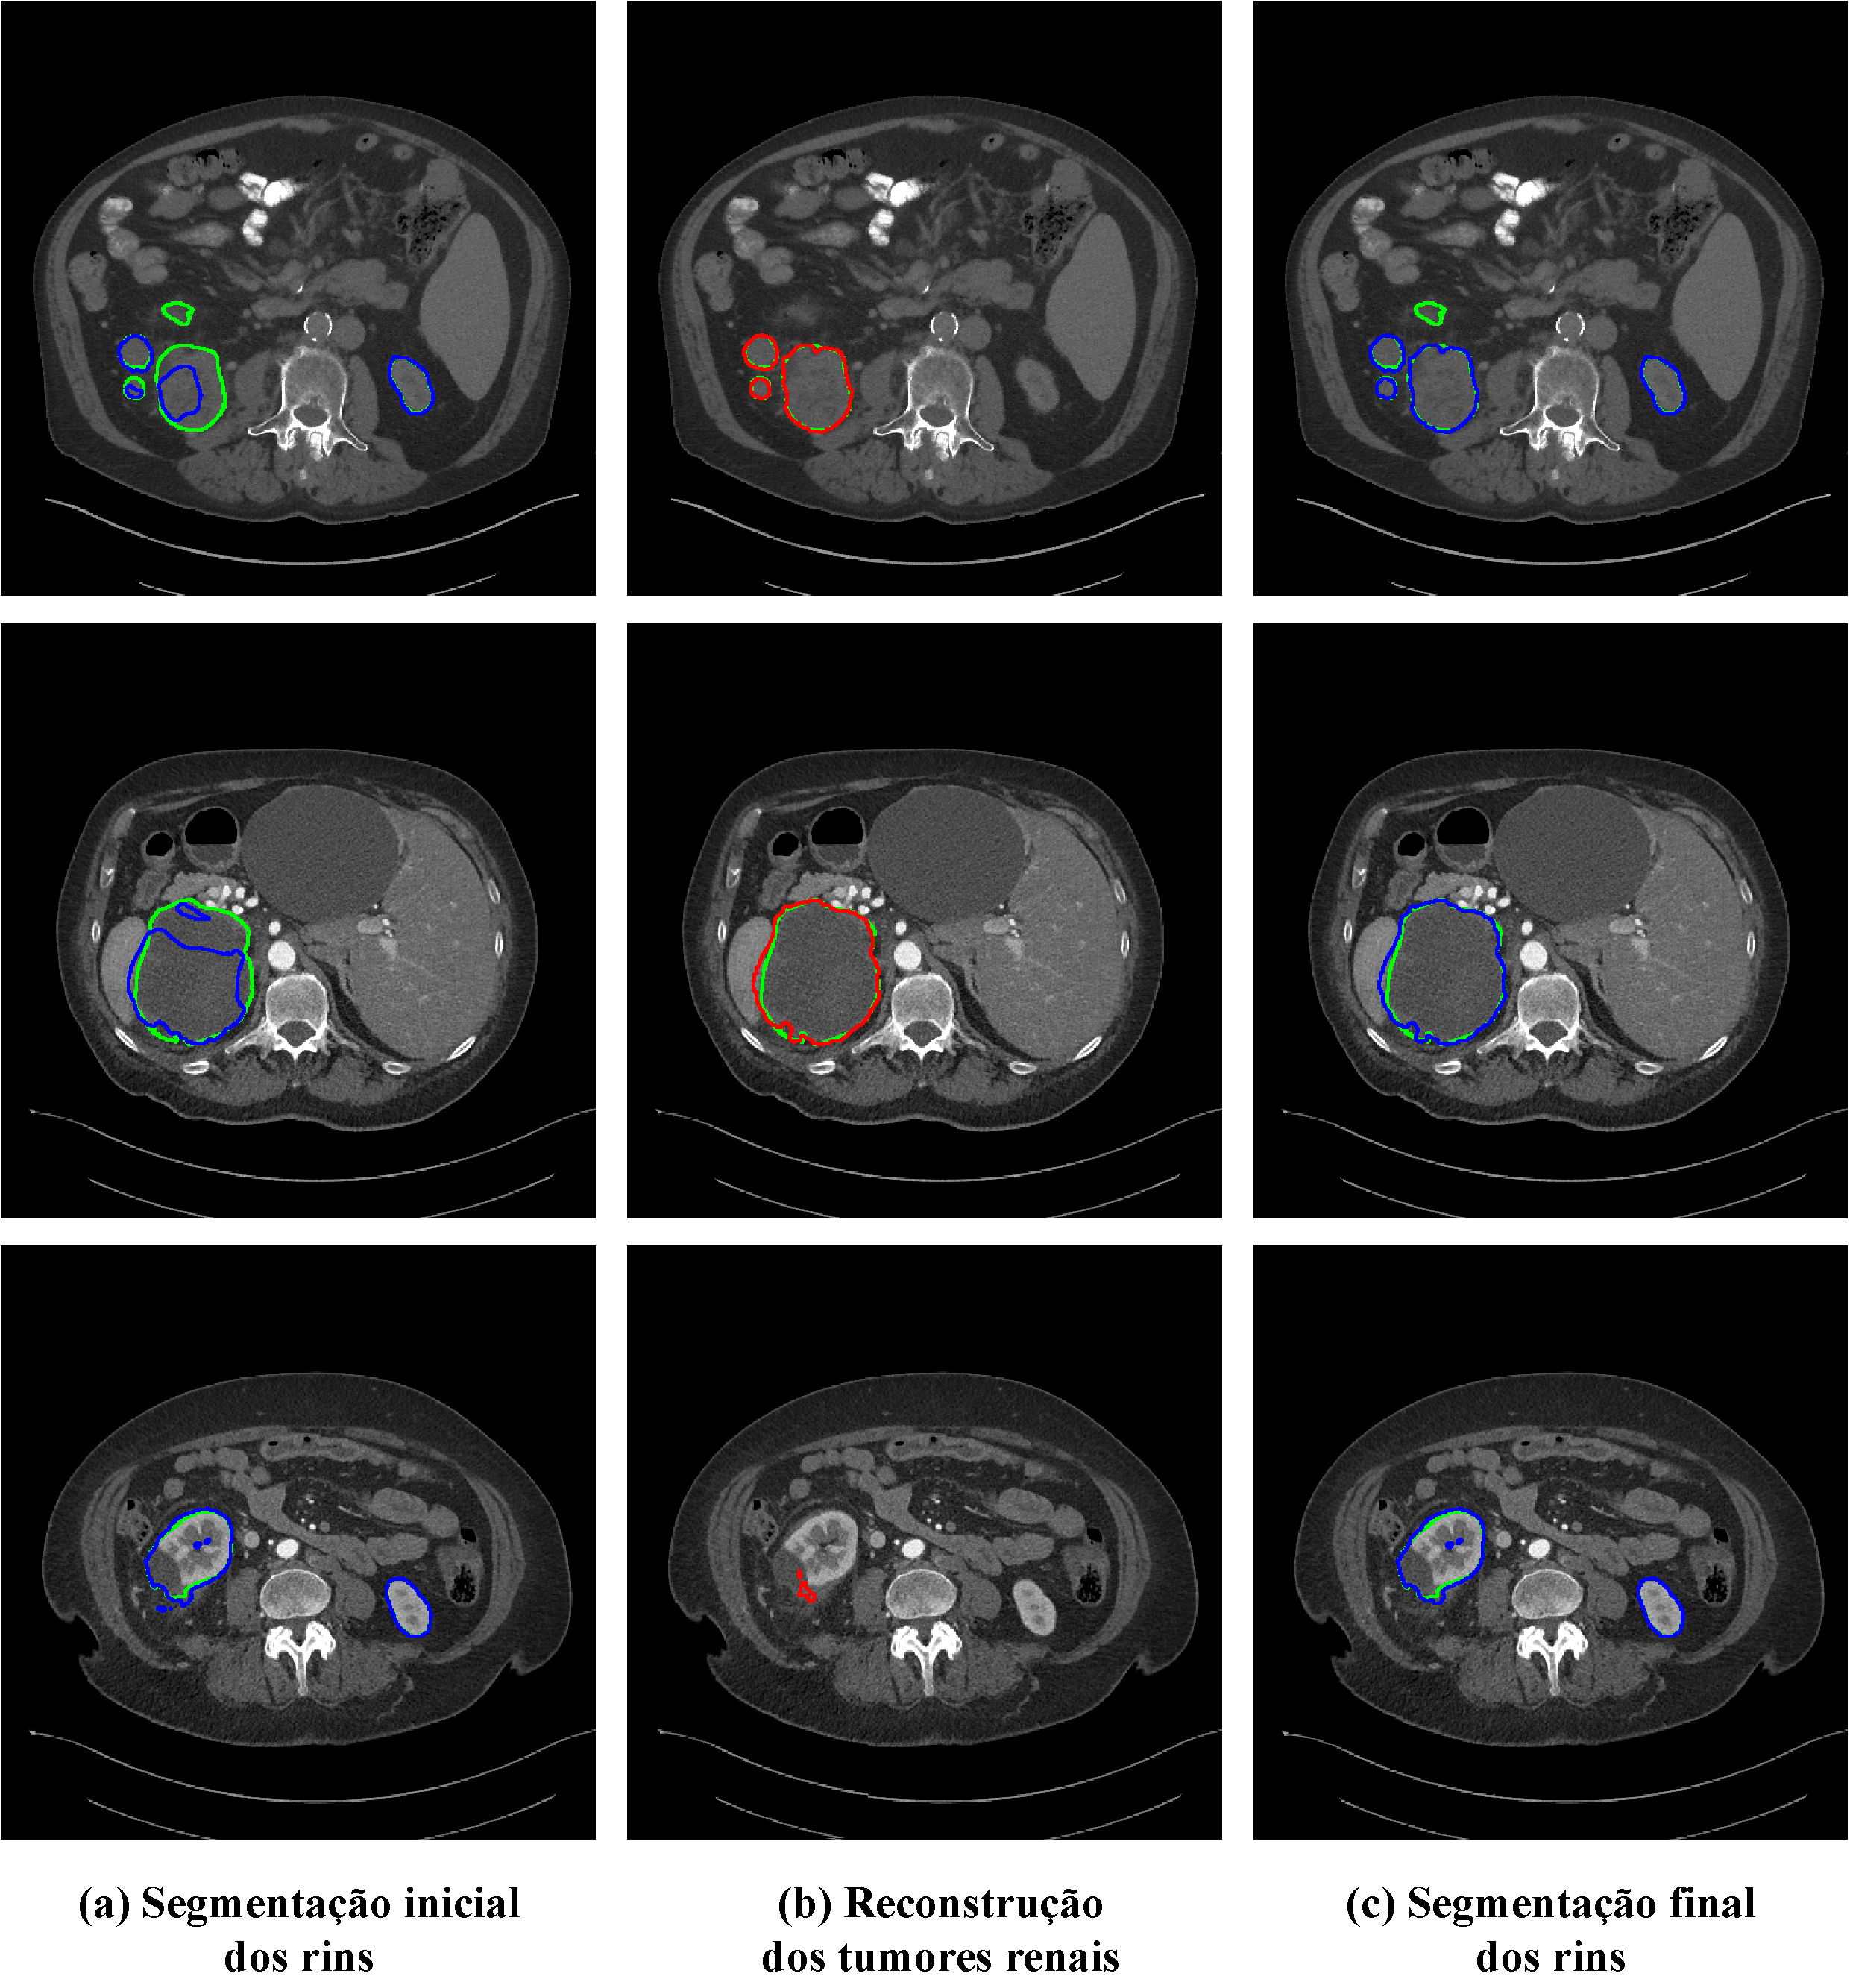
\includegraphics[width=0.98\textwidth]{figuras/res-seg-rins-final.pdf}
    \label{fig:res-final-rins}
    \legend{Fonte: Elaborado pela autora.}
\end{figure}

Vale destacar o último caso (imagens inferiores), em que alguns falsos positivos segmentados foram observados na etapa inicial de segmentação renal (Figura~\ref{fig:res-final-rins} (a) inferior). No entanto, foram removidos após a aplicação do pós-processamento (manter os dois maiores elementos). Portanto, acredita-se que este conjunto de etapas seja capaz de contribuir para melhorar o resultado da segmentação de rins.


%Observando a etapa de manter apenas o maior objeto, garante-se uma melhora em relação ao Dice e especificidade, ou seja, há menos falsos positivos e uma segmentação mais precisa. Apesar de haver uma perda na sensibilidade, vale lembrar que as métricas são medidas por pixels, ou seja, existem mais números de pixels pertencentes a classe de não esôfago do que esôfago, então qualquer melhora na especificidade (acertar os casos negativos) melhora significativamente o valor de Dice.

\subsection{Redução de Falsos Positivos para os Tumores Renais}
\label{sec:resultados-reducao-falsos-positivos-tumores-renais}

Esta etapa completa o método proposto para segmentação de tumores renais. Para isso, são usadas as segmentações das etapas anteriores obtidas, conforme descrito na Seção~\ref{sec:resultados-reducao-falsos-positivos-rins}. Com as segmentações obtidas, foi feita a intersecção da segmentação final dos rins com a etapa de reconstrução dos tumores renais para extrair apenas a região que contém os tumores, removendo assim parte dos falsos positivos adquiridos na reconstrução dos tumores. Finalmente, os resultados dessa etapa são passados pela etapa de pós-processamento para reduzir os falsos positivos que não foram removidos na etapa anterior. 

O pós-processamento consistiu na remoção de estruturas segmentadas sem informação contextual suficiente para representar as regiões dos tumores renais, ou seja, elementos com menos de três fatias contínuas (Seção~\ref{sec:metodo-reducao-falsos-positivos-tumores-renais}). Os resultados após o pós-processamento estão descritos na Tabela~\ref{tab:seg-final-tumores-renais}. A segmentação final atingiu 84,06\% de Dice, 75,04\% de Jaccard, 99,94\% de acurácia, 88,33\% de sensibilidade e 99,95\% de especificidade.

\begin{table}[!ht]
\caption{Resultados da etapa de segmentação final dos tumores renais.}
\label{tab:seg-final-tumores-renais}
\centering
\begin{tabular}{c|c|c|c|c|c}
\hline
Resultado Final  & Dice(\%)                      & Jacc(\%)                      & Acc(\%) & Sen(\%)                       & Esp(\%) \\ \hline
2D               & 73,62                          & 61,21                          & 99,89    & 81,03                          & 99,91    \\ \hline
2.5D             & 84,06                          & 75,04                          & 99,94    & 88,33                          & 99,95    \\ \hline
\textit{P-value} & \cellcolor[HTML]{C0C0C0}0,0000 & \cellcolor[HTML]{C0C0C0}0,0000 & 0,3680   & \cellcolor[HTML]{C0C0C0}0,0000 & 0,4275   \\ \hline
\end{tabular}
\end{table}

Em termos estatísticos, a segmentação final dos tumores renais usando as abordagens 2D e 2.5D apresentou um \textit{p-value} igual a 0 para as métricas Dice, Jaccard e sensibilidade. Portanto, comprova que existe uma diferença significativa entre as segmentações finais, visto que a hipótese nula foi rejeitada. Isso demonstra que as segmentações finais usando a abordagem 2.5D são mais precisas, com menos falsos positivos e mais regiões de tumores. Uma vez que, as métricas descritas (Dice, Jaccard e sensibilidade) indicam a capacidade de identificar regiões de tumores e a semelhança entre os objetos em estudo.

Além disso, pode-se observar que houve melhorias consideráveis nas métricas Dice, Jaccard e sensibilidade em relação às segmentações iniciais dos candidatos a tumores renais (Seção~\ref{sec:resultados-candidatores-tumores-renais-regiao-renal} e~\ref{sec:resultados-candidatores-tumores-renais-regiao-abdominal}). Isso comprova a importância das etapas anteriores para a obtenção de resultados expressivos. Portanto, devido à melhora significativa nos resultados finais, o trabalho dos especialistas para analisar todos os elementos segmentados é reduzido.

Três casos aplicando as etapas para obter a segmentação final dos tumores renais são apresentados na Figura~\ref{fig:res-final-tumores-renais}. Primeiramente, pode-se observar que a segmentação de candidatos a tumores renais na região renal (Figura~\ref{fig:res-final-tumores-renais} (a)) não foi capaz de segmentar com precisão as regiões dos tumores. Além disso, muitas regiões renais não foram segmentadas na etapa de segmentação inicial dos rins, o que acabou comprometendo o desempenho do modelo, uma vez que ficou impossibilitado de segmentar mais regiões tumorais. No entanto, a etapa de segmentação de candidatos a tumores renais na região abdominal (Figura~\ref{fig:res-final-tumores-renais} (b)) compensa a deficiência da segmentação inicial dos rins e candidatos a tumores renais na região renal, permitindo a segmentação de mais regiões tumorais. Isso é possível porque esta etapa analisa mais informações contextuais em uma região mais ampla (abdominal). 

\begin{figure}[!ht]
    \centering
    \caption{Etapas da segmentação dos tumores renais. Marcação do especialista (verde) e segmentação do método (vermelho).}
    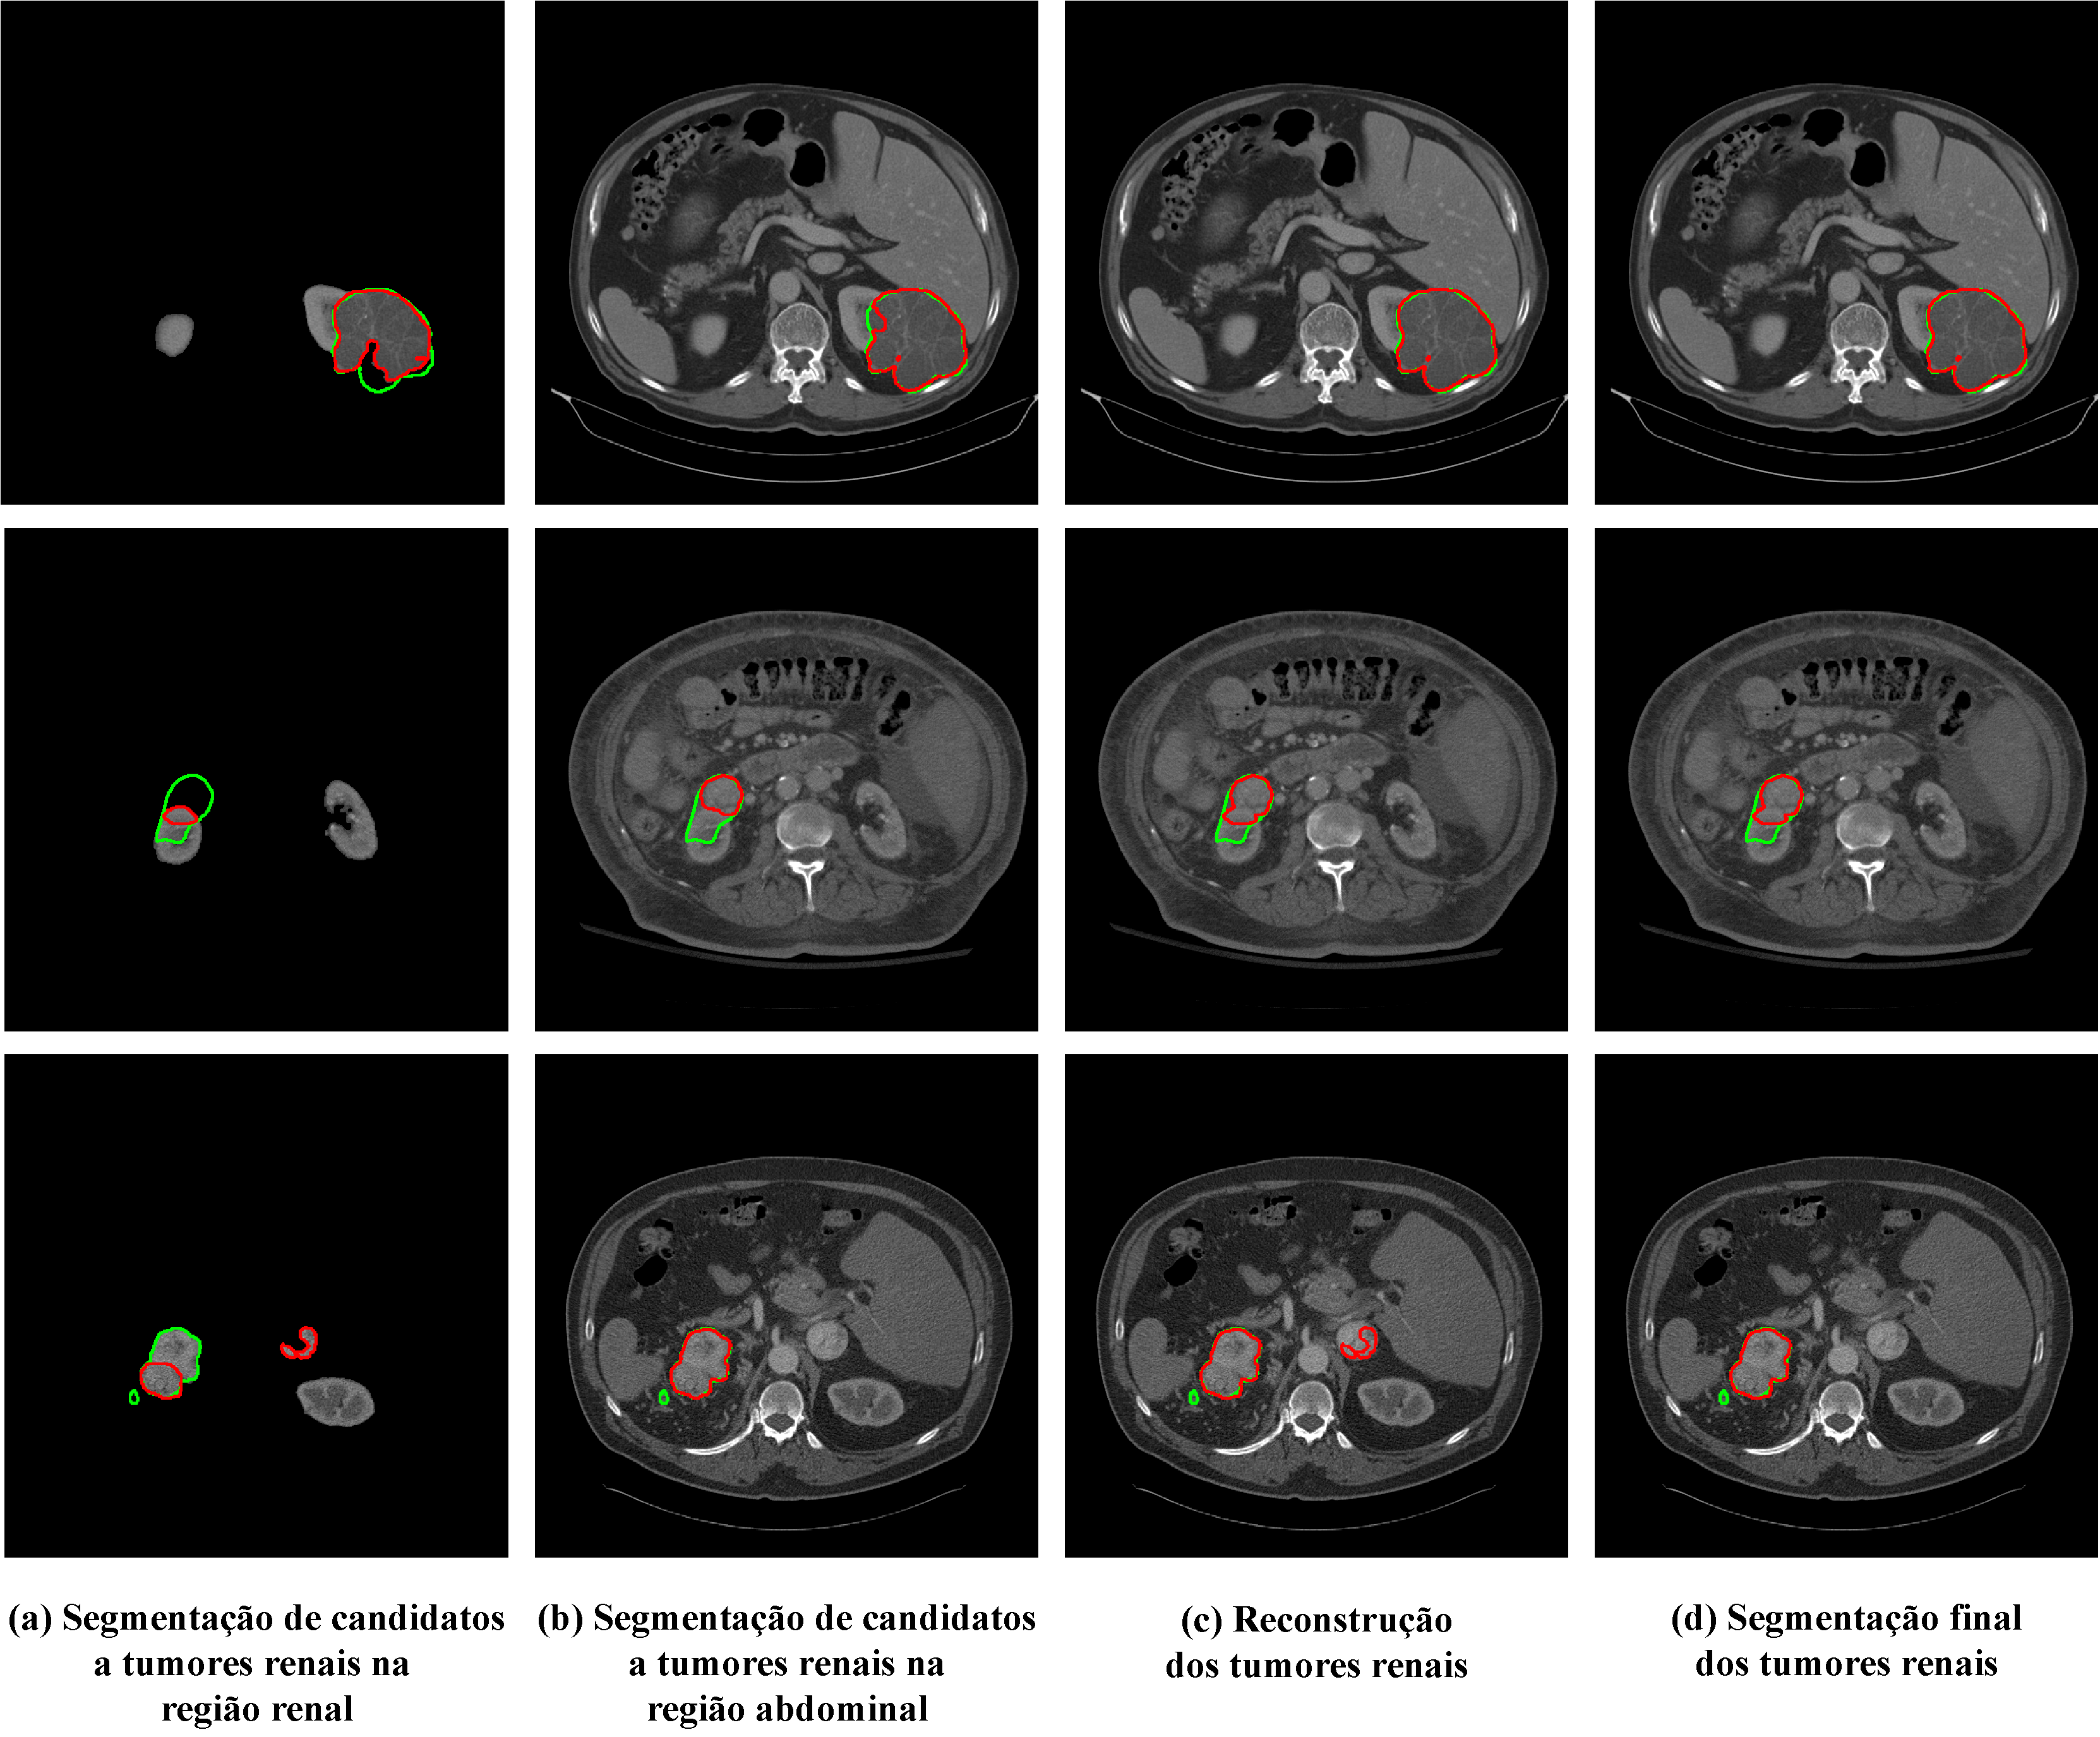
\includegraphics[width=1\textwidth]{figuras/res-seg-tumores-renais-final.pdf}
    \label{fig:res-final-tumores-renais}
    \legend{Fonte: Elaborado pela autora.}
\end{figure}
\FloatBarrier

Posteriormente, a etapa de reconstrução de tumores renais (Figura~\ref{fig:res-final-tumores-renais} (c)) combinou as etapas de segmentação de candidatos a tumores renais na região renal e abdominal. Isso levou a uma segmentação mais precisa da região tumoral, pois regiões tumorais não segmentadas no primeiro estágio foram segmentadas no segundo estágio, agregando os resultados. Finalmente, a segmentação final dos tumores é mostrada na Figura~\ref{fig:res-final-tumores-renais} (d). Pode-se analisar que mais tecidos das regiões tumorais foram incluídos devido à etapa de reconstrução do tumor.

Por fim, vale destacar o último caso (imagens inferiores) da Figura~\ref{fig:res-final-tumores-renais}. No qual pode-se observar que na etapa de segmentação dos candidatos a tumores renais na região renal (Figura~\ref{fig:res-final-tumores-renais} (a) inferior), as regiões tumorais foram segmentadas, mas também falsos positivos. Entretanto, foram eliminados após a aplicação do pós-processamento (remoção de elementos descontínuos). Portanto, acredita-se que todas as etapas foram importantes para melhorar a segmentação dos tumores.

\subsection{Método Proposto com/sem Balanceamento de Fatias}
\label{sec:com-sem-balanceamento-fatias}

Após os experimentos usando abordagens 2D e 2.5D, foram realizados mais alguns experimentos para validar as demais etapas do método proposto. Primeiramente, foi verificada a eficácia da técnica de balanceamento de fatias no conjunto de treinamento e validação. Para isso, foi realizado um experimento com e sem balanceamento de fatias no método proposto, no qual, ao invés de usar a estratégia de balanceamento de fatias, os modelos foram treinados e validados usando todas as fatias dos volumes de TCs. Posteriormente, todas as outras etapas do método proposto foram aplicadas com base neste experimento. Os resultados finais do método proposto com e sem balanceamento proporcional são apresentados na Tabela~\ref{tab:com-sem-balanceamento}. Além disso, é mostrado o tempo de treinamento para cada época dos modelos (ResUNet 2.5D e DeepLabv3+ 2.5D). Na segmentação dos tumores renais é apresentado o resultado da soma dos tempos de treinamento dos modelos para segmentar candidatos a tumores renais na região renal e abdominal.

\begin{table}[!ht]
\caption{Resultado do método proposto com/sem balanceamento de fatias.}
\label{tab:com-sem-balanceamento}
\doublespacing
\centering
\resizebox{\columnwidth}{!}{
\begin{tabular}{cl|c|c|c|c|c|c}
\hline
\multicolumn{1}{c|}{Segmentação}                                                                                 & \multicolumn{1}{c|}{Técnica} & Dice(\%)                      & Jacc(\%)                      & Acc(\%) & Sen(\%)                       & Esp(\%) & T. por época \\ \hline
\multicolumn{1}{l|}{}                                                                                            & Todas as fatias              & 43,79                          & 32,11                          & 99,63    & 77,00                          & 99,65    & -            \\ \cline{2-8} 
\multicolumn{1}{l|}{\multirow{-2}{*}{\begin{tabular}[c]{@{}l@{}}Reconstrução dos\\ Tumores Renais\end{tabular}}} & Balanceado                   & 68,20                          & 57,17                          & 99,90    & 90,33                          & 99,91    & -            \\ \hline
\multicolumn{1}{c|}{}                                                                                            & Todas as fatias              & 92,96                          & 87,38                          & 99,84    & 93,05                          & 99,92    & 1h 01m 52s            \\ \cline{2-8} 
\multicolumn{1}{c|}{\multirow{-2}{*}{Rins}}                                                                      & Balanceado                   & 97,45                          & 95,05                          & 99,95    & 98,44                          & 99,96    & 33m 29s            \\ \hline
\multicolumn{1}{c|}{}                                                                                            & Apenas fatias com rins       & 62,03                          & 49,15                          & 99,82    & 75,99                          & 99,85    & 46m 03s            \\ \cline{2-8} 
\multicolumn{1}{c|}{\multirow{-2}{*}{Tumores Renais}}                                                            & Balanceado                   & 84,06                          & 75,04                          & 99,94    & 88,33                          & 99,95    & 24m 33s            \\ \hline
\multicolumn{2}{c|}{\textit{P-value}}                                                                                                           & \cellcolor[HTML]{C0C0C0}0,0000 & \cellcolor[HTML]{C0C0C0}0,0000 & 0,0690   & \cellcolor[HTML]{C0C0C0}0,0000 & 0,0969   & -            \\ \hline
\end{tabular}
}
\end{table}

Pode-se observar que a abordagem proposta com balanceamento de fatias produz melhorias significativas em todas as colunas em comparação com a abordagem sem balanceamento de fatias. Inclusive o tempo com balanceamento é inferior, pois tem menos fatias que a abordagem sem balanceamento. Analisando a métrica sensibilidade entre as abordagens, pode-se verificar que sofreu um impacto negativo em relação à abordagem com balanceamento de fatias. Isso acontece porque, sem aplicar o balanceamento de fatias, os modelos terão como entrada mais fatias de fundo (sem rim, sem tumores, dependendo do modelo) do que fatias com o objeto de interesse (rins ou tumores). Dessa forma, o modelo tende a aprender mais fatias de fundo e não consegue segmentar com precisão o objeto de interesse, portanto, o modelo tem baixa sensibilidade e, consequentemente, resultados baixos para Dice e Jaccard.

Além disso, estatisticamente, obteve-se um \textit{p-value} de 0,0034 na acurácia em relação à reconstrução de tumores e um \textit{p-value} igual a 0 para as métricas Dice, Jaccard e sensibilidade em relação a todas as abordagens com/sem balanceamento de fatias e, portanto, a hipótese nula foi rejeitada. Portanto, com os resultados experimentais foi possível comprovar que a técnica de balanceamento de fatias é fundamental para a obtenção de resultados mais consistentes na segmentação dos rins e segmentação e reconstrução de tumores renais. Essa melhora se deve à capacidade do balanceamento detectar fatias com e sem tumores, possibilitando segmentar mais regiões de interesse e minimizar falsos positivos.

%-- Reconstrução de tumores 0,0034 acurácia

\subsection{Método Proposto com Distribuição Aleatória e Proporcional da Base de Imagens}
\label{sec:distribuicao-proporcional-grupos-tumores}

O próximo experimento realizado foi relacionado a etapa da distribuição proporcional da base de imagens. Para validar essa etapa, o conjunto de teste permaneceu o mesmo e os modelos de segmentação e reconstrução foram treinados com outro conjunto de treino e validação distribuídos aleatoriamente. As demais etapas do método proposto foram aplicadas posteriormente. Os resultados finais do método proposto com distribuição aleatória e proporcional são apresentados na Tabela~\ref{tab:aleatorio-distribuidos}. Também são apresentados o tempo de treinamento para cada época dos modelos (ResUNet 2.5D e DeepLabv3+ 2.5D). Na segmentação dos tumores renais, é apresentado o resultado da soma dos tempos de treinamento dos modelos para segmentar candidatos a tumores renais na região renal e abdominal.

\begin{table}[!ht]
\caption{Resultado do método proposto com distribuição aleatória e proporcional.}
\label{tab:aleatorio-distribuidos}
\doublespacing
\centering
\resizebox{\columnwidth}{!}{
\begin{tabular}{cl|c|c|c|c|c|c}
\hline
\multicolumn{1}{c|}{Segmentação}                                                                                 & \multicolumn{1}{c|}{Técnica} & Dice(\%)                      & Jacc(\%)                      & Acc(\%) & Sen(\%)                       & Esp(\%) & T. por época \\ \hline
\multicolumn{1}{l|}{}                                                                                            & Aleatório                    & 53,39                          & 40,78                          & 99,78    & 82,22                          & 99,81    & -            \\ \cline{2-8} 
\multicolumn{1}{l|}{\multirow{-2}{*}{\begin{tabular}[c]{@{}l@{}}Reconstrução dos\\ Tumores Renais\end{tabular}}} & Distribuição proporcional    & 68,20                          & 57,17                          & 99,90    & 90,33                          & 99,91    & -            \\ \hline
\multicolumn{1}{c|}{}                                                                                            & Aleatório                    & 94,18                          & 90,06                          & 99,90    & 94,44                          & 99,95    & 34m 33s            \\ \cline{2-8} 
\multicolumn{1}{c|}{\multirow{-2}{*}{Rins}}                                                                      & Distribuição proporcional    & 97,45                          & 95,05                          & 99,95    & 98,44                          & 99,96    & 33m 29s            \\ \hline
\multicolumn{1}{c|}{}                                                                                            & Aleatório                    & 71,29                          & 59,17                          & 99,89    & 80,64                          & 99,91    & 27m 14s           \\ \cline{2-8} 
\multicolumn{1}{c|}{\multirow{-2}{*}{Tumores Renais}}                                                            & Distribuição proporcional    & 84,06                          & 75,04                          & 99,94    & 88,33                          & 99,95    & 24m 33s             \\ \hline
\multicolumn{2}{c|}{\textit{P-value}}                                                                                                           & \cellcolor[HTML]{C0C0C0}0,0000 & \cellcolor[HTML]{C0C0C0}0,0000 & 0,1152   & \cellcolor[HTML]{C0C0C0}0,0000 & 0,1605   & -            \\ \hline
\end{tabular}
}
\end{table}

A partir dos resultados obtidos, é possível ver a importância da etapa de distribuição proporcional, não só por ter obtido resultados melhores do que com a aplicação da distribuição aleatória, mas também por atingir um \textit{p-value} igual a 0 para várias métricas (Dice, Jaccard e sensibilidade), revelando-se significativamente diferentes. Portanto, esta etapa garante que os modelos sejam equilibrados e obtenham um melhor desempenho, além de ser importante para o sucesso das demais etapas do método proposto.

\subsection{Segmentação de Rins sem/com a Etapa de Reconstrução de Tumores Renais}
\label{sec:segmentacao-rins-sem-reconstrucao-tumoral}

Neste experimento, o foco foi avaliar a etapa de reconstrução de tumores renais do método proposto para segmentação de rins. Basicamente, a etapa de reconstrução tumoral foi excluída para verificar o impacto nos resultados da segmentação renal. Vale ressaltar que todas as configurações experimentais e demais etapas foram aplicadas. Os resultados são apresentados na Tabela~\ref{tab:res-segmentacao-rins-sem-reconstrucao-tumoral}.

\begin{table}[!ht]
\caption{Resultados da segmentação de rins com e sem a etapa de reconstrução tumoral.}
\label{tab:res-segmentacao-rins-sem-reconstrucao-tumoral}
\centering
\onehalfspacing
\resizebox{\columnwidth}{!}{
\begin{tabular}{c|c|c|c|c|c}
\hline
Segmentação de Rins                & Dice(\%) & Jacc(\%) & Acc(\%) & Sen(\%)                       & Esp(\%) \\ \hline
Sem Reconstrução de Tumores Renais & 97,11     & 94,44     & 99,94    & 97,57                          & 99,97    \\ \hline
Com Reconstrução de Tumores Renais & 97,45     & 95,05     & 99,95    & 98,44                          & 99,96    \\ \hline
\textit{P-value}                   & 0,2794    & 0,1550    & 0,8767   & \cellcolor[HTML]{C0C0C0}0,0011 & 0,9375   \\ \hline
\end{tabular}
}
\end{table}

Analisando os resultados das métricas de avaliação, pode-se notar que os melhores resultados da segmentação de rins é aplicando também a etapa de reconstrução tumoral. Essa etapa é capaz de recuperar regiões consideráveis de tumores, que por sua vez também são regiões renais e possivelmente não foram inicialmente segmentadas. Portanto, ao aplicar a reconstrução tumoral, as regiões renais também são reconstruídas, delimitando melhor os contornos renais. Estatisticamente, obteve-se um \textit{p-value} de 0,0011 para a métrica de sensibilidade em relação às abordagens comparadas. Isso significa que o uso da etapa de reconstrução tumoral tem impacto positivo na obtenção de mais regiões da classe positiva (rins). Portanto, acredita-se que essa etapa é válida para obter resultados mais precisos para a segmentação renal.

\subsection{Segmentação de Tumores Renais aplicando a Máscara do Método/Especialista}
\label{sec:segmentacao-tumores-mascara-metodo-especialista}

No último experimento, a segmentação de tumores renais foi analisada usando diferentes abordagens de imagens de entrada para o método. Para validar isso, apenas as formas de entrada para a segmentação de candidatos a tumores renais na região renal foram usadas para estudo. As demais etapas não foram utilizadas para não causar impacto no estudo avaliado em questão. Portanto, o objetivo deste experimento é investigar o impacto da segmentação de tumores quando a máscara renal marcada pelo especialista é aplicada como entrada da rede e como as demais etapas são refletidas.

\begin{table}[!ht]
\caption{Resultados da segmentação de tumores renais aplicando a máscara do método e do especialista.}
\label{tab:res-segmentacao-tumores-mascara-metodo-especialista}
\centering
\onehalfspacing
\resizebox{\columnwidth}{!}{
\begin{tabular}{c|c|c|c|c|c}
\hline
Segmentação de Tumores Renais & Dice(\%)                      & Jacc(\%)                      & Acc(\%) & Sen(\%)                       & Esp(\%) \\ \hline
Máscara do Especialista       & 84,95                          & 75,06                          & 99,68    & 84,44                          & 99,80    \\ \hline
Máscara do Método             & 81,02                          & 69,66                          & 99,93    & 80,52                          & 99,97    \\ \hline
\textit{P-value}              & \cellcolor[HTML]{C0C0C0}0,0010 & \cellcolor[HTML]{C0C0C0}0,0001 & 0,0738   & \cellcolor[HTML]{C0C0C0}0,0011 & 0,1136   \\ \hline
\end{tabular}
}
\end{table}

As duas abordagens avaliadas foram: aplicar a máscara proveniente da segmentação inicial dos rins (etapa anterior) como entrada da rede; e usar a máscara renal marcada pelo especialista como entrada da rede. Os resultados dessas abordagens são apresentados na Tabela~\ref{tab:res-segmentacao-tumores-mascara-metodo-especialista}. É perceptível que os resultados usando como entrada da rede a máscara do especialista apresentaram resultados superiores. Além disso, em termos estatísticos também comprovam que as abordagens são significativamente diferentes.

A partir disto, é possível tirar conclusões sobre a segmentação inicial dos rins obtida pelo método proposto. Em que, embora 96,37\% de Dice seja obtido na segmentação inicial dos rins (Tabela~\ref{tab:seg-inicial-rins}), partes de regiões renais que também são tumores não são segmentadas. Portanto, usando a máscara dos rins da segmentação inicial dos rins, não foi possível segmentar maiores regiões tumorais devido à perda de regiões renais. No entanto, resultados superiores foram produzidos aplicando a máscara do especialista ao mesmo modelo de segmentação (DeepLabv3+ 2.5D). Portanto, é possível concluir que o modelo de segmentação de tumores apresenta bom desempenho, pois o que causa resultados inferiores é somente quando as regiões renais que possuem tumores não são visíveis como áreas para segmentação.

Entretanto, é importante destacar que a deficiência da segmentação de rins é suprida com as demais etapas do método proposto. Em que as regiões não segmentadas inicialmente são reconstruídas usando a etapa de reconstrução dos tumores renais. Mediante isso, os resultados finais para a segmentação de tumores (84,06\% de Dice, na Tabela~\ref{tab:seg-final-tumores-renais}) são equiparáveis aos resultados quando não há perda de regiões renais/tumorais. Mais uma vez, é notável como as etapas do método proposto são essenciais e robustas, o que acaba impactando nos bons resultados para a segmentação de rins e tumores.

%A partir disto, é possível tirar conclusões sobre a qualidade da segmentação de rins obtida pelo método proposto e verificar as demais etapas para suprir possíveis deficiências da segmentação de rins.

\section{Diversos Experimentos Testados}
\label{sec:experimentos-testados}

Finalmente, esta última seção descreve um resumo dos principais experimentos realizados na elaboração do método proposto. A Tabela~\ref{tab:diversos-experimentos} apresenta o resumo dos principais pré-processamentos, arquiteturas, codificadores e abordagens aplicadas. Os diversos experimentos foram aplicados em diferentes etapas do método e foram feitas combinações entre eles.

\begin{table}[!ht]
\caption{Resumo dos diversos experimentos testados.}
\label{tab:diversos-experimentos}
\centering
\onehalfspacing
\resizebox{\columnwidth}{!}{
\begin{tabular}{c|c|c|c}
\hline
Pré-processamentos                                                                                               & Arquiteturas                                                                                               & Codificadores                                                                                                                                                                                        & Abordagens                                                            \\ \hline
\begin{tabular}[c]{@{}c@{}}CLAHE, bilateral, média,\\ equalização do histograma\\ e unsharp masking\end{tabular} & \begin{tabular}[c]{@{}c@{}}UNet, UNet++,\\ DeepLabv3, DenseUNet\\ e Pyramid Attention Network\end{tabular} & \begin{tabular}[c]{@{}c@{}}AlexNet, DenseNet, ResNet-18,\\ ResNet-34, ResNet-50, ResNet-152,\\ ResNeXt, SqueezeNet, Xception,\\ Inception, DPN-98, EfficientNet-B3\\ e EfficientNet-B7\end{tabular} & \begin{tabular}[c]{@{}c@{}}2D, 2.5D\\ (com 5 e 7 fatias)\end{tabular} \\ \hline
\end{tabular}
}
\end{table}

Na primeira coluna, podem ser vistos os principais pré-processamentos que foram aplicados na etapa inicial do método proposto. Todos eles foram testados individualmente e em conjunto com o objetivo de melhorar as imagens usadas no método, visando aprimorar o desempenho de segmentação. A segunda coluna contém as arquiteturas de rede que foram testadas para segmentação de rins e candidatos a tumores renais, nas quais pode-se observar que foram usadas desde arquiteturas clássicas como a U-Net até arquiteturas de última geração como DeepLabv3 e \textit{Pyramid Attention Network}~\cite{li2018pyramid}. A terceira coluna mostra os codificadores que foram testados nas arquiteturas descritas.

A última coluna, mostra as abordagens 2D e 2.5D. No caso da abordagem 2.5D, foram testados com 5 e 7 fatias. \textit{O data augmentation offline} também foi testado, mas desvantagens como memória e tempo de treinamento adicionais e alto custo computacional foram encontrados. De qualquer forma, \textit{data augmentation online} apresentou resultados superiores com baixo custo computacional em relação aos outros. Por fim, é importante destacar que para cada um dos experimentos foram aplicadas diversas combinações entre eles. Em geral, como pode ser visto, durante o desenvolvimento do método proposto atual uma série de testes foram realizados. No entanto, os experimentos descritos não superaram os resultados atuais, apresentando resultados inferiores a 90,12\% e 66,7\% de Dice na segmentação de rins e tumores, respectivamente, levando-se em consideração a melhor combinação.

\section{Considerações Finais}
\label{considerações-finais-resultados}

Neste capítulo, os resultados obtidos pelos experimentos realizados no desenvolvimento do método proposto foram apresentados e discutidos. Além disso, mais alguns experimentos foram realizados a fim de validar as etapas do método proposto.

No próximo capítulo serão apresentados os estudos de casos, também será feita uma comparação com os trabalhos descritos na literatura, visando contextualizar a relevância da pesquisa desenvolvida neste trabalho. Por fim, serão descritos os principais aspectos e limitações encontrados após a análise das etapas propostas.
